%!TEX root = ../terrainbook.tex

\graphicspath{{spatialextent/}}

\chapter{The spatial extent of a point cloud}
\label{chap:spatialextent}

\begin{figure}[h]
  \centering
  \begin{subfigure}[b]{0.21\linewidth}
    \centering
    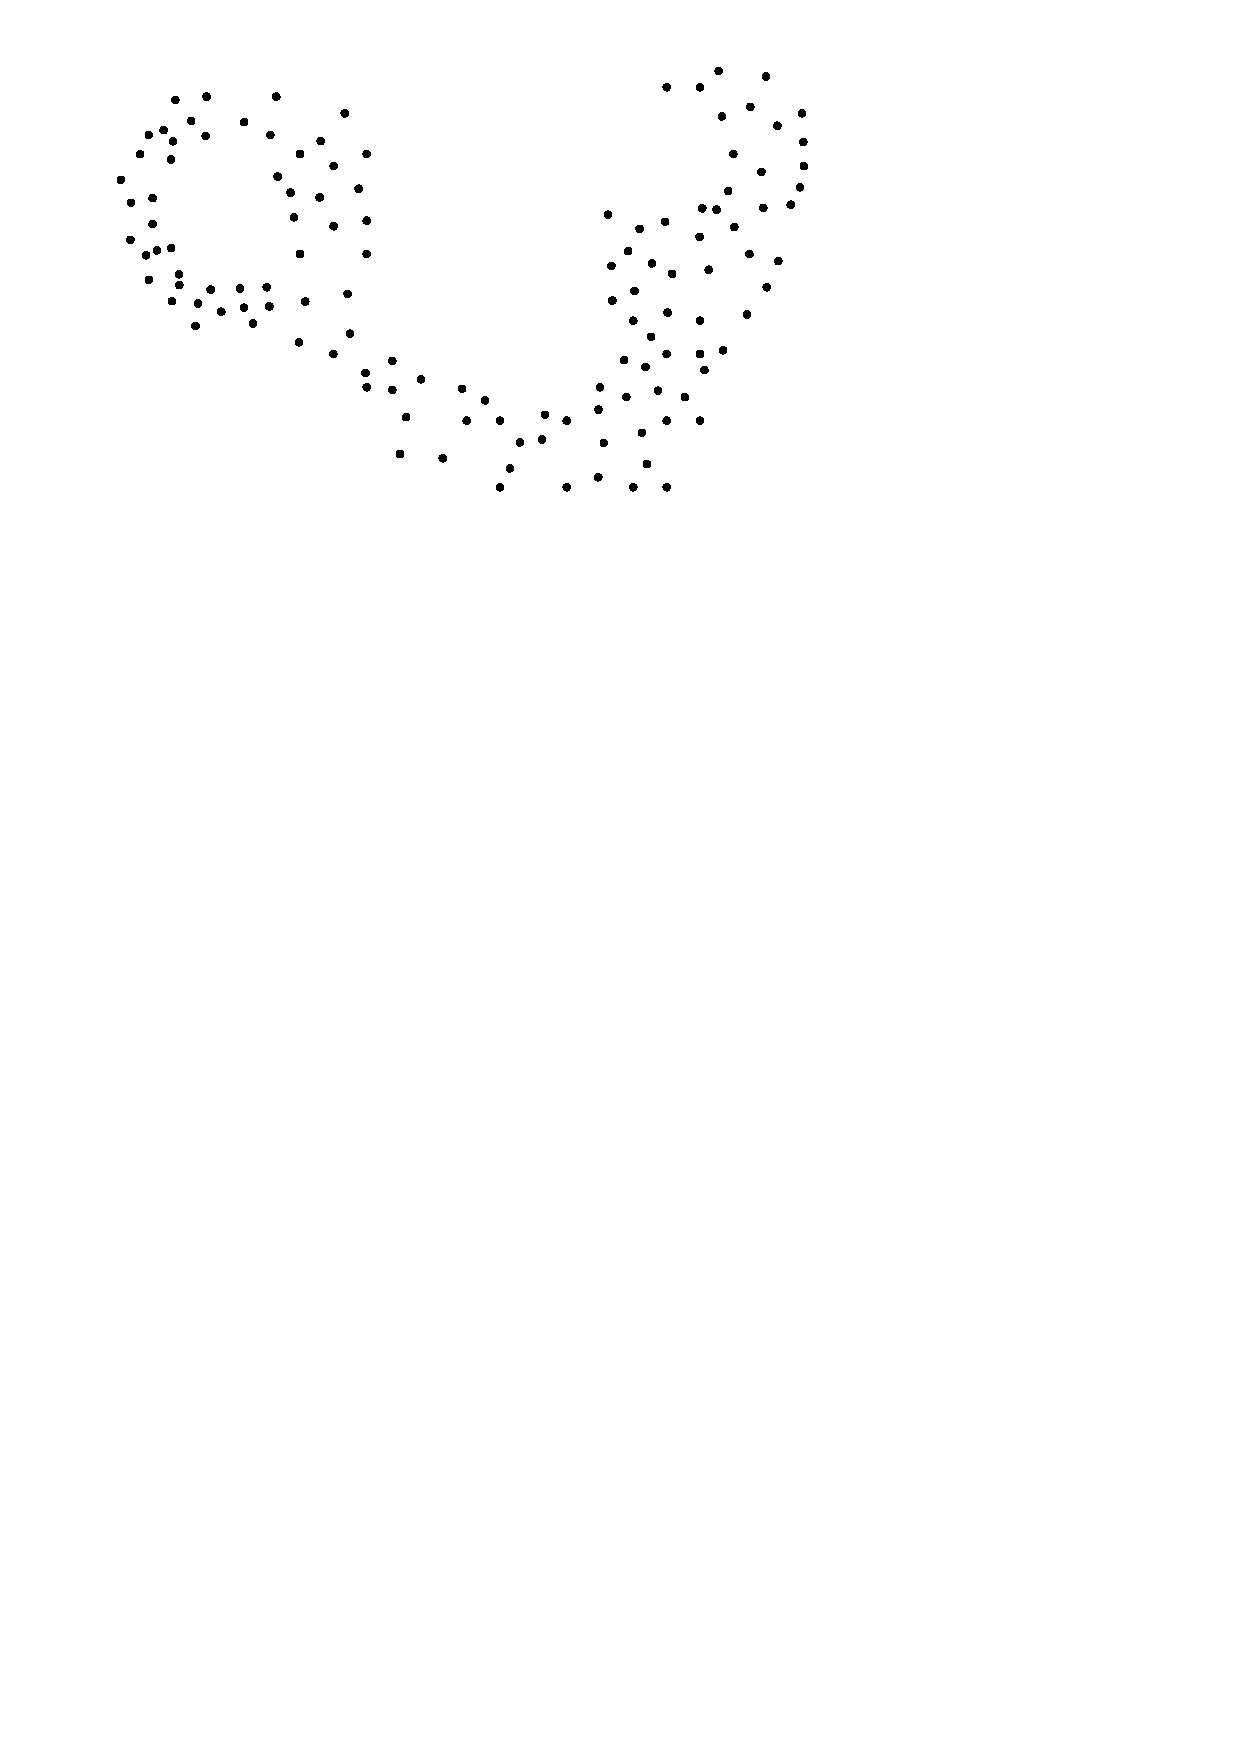
\includegraphics[page=1,width=\textwidth]{figs/idea.pdf}
    \caption{A set of points in $\mathbb{R}^2$}
  \end{subfigure}%
  \qquad
  \begin{subfigure}[b]{0.21\linewidth}
    \centering
    \includegraphics[page=2,width=\textwidth]{figs/idea.pdf}
    \caption{Its convex hull}
  \end{subfigure}
  \qquad
  \begin{subfigure}[b]{0.21\linewidth}
    \centering
    \includegraphics[page=3,width=\textwidth]{figs/idea.pdf}
    \caption{A $\chi$-shape}
  \end{subfigure}%
  \qquad
  \begin{subfigure}[b]{0.21\linewidth}
    \centering
    \includegraphics[page=4,width=\textwidth]{figs/idea.pdf}
    \caption{An $\alpha$-shape}
  \end{subfigure}
\caption{Different methods to obtain the spatial extent of a given set of points in the plane.}
\label{fig:ideas}  
\end{figure}

Given a point cloud, one operation that practitioners need to perform is to define the spatial extent of the dataset.
That is, they need to define the shape of the region that best abstracts the set of points; in the context of terrains this region is often in two dimensions.
% , which is represented by a one or more polygons,
This is useful for instance to calculate the area covered by a dataset, to convert it to other formats (\eg\ raster), to get a quick overview of several datasets it is faster to load a few polygons and not billions of points, etc.

%

The spatial extent is often called: envelope, hull, concave hull, or footprints.
It is important to notice that the spatial extent is not uniquely defined and can a vague concept, as Figure~\ref{fig:ideas} shows there are several potential regions for a rather simple set of points, and most of these could be considered `correct' by a human.

%

We present in this chapter a few methods/algorithms that are used in practice to define the spatial extent of a set of points in $\mathbb{R}^2$, which implies that the points in a point cloud are projected to the plane.

% TODO : linear approximation only here


%%%%%%%%%%%%%%%%%%%%
%
\section{Properties of the region}
\label{sec:properties}

Let $S$ be a set of points in $\mathbb{R}^2$, and $R(S)$ the region that characterise the spatial extent of $S$.
The region is potentially formed by a set of polygons (if $S$ forms two distinct clusters for instance) and in practice most algorithms will computer a linear approximation of $R(S)$, so the polygons will have straight edges as boundaries.

To evaluate the different algorithms, we list here different properties that one must consider when defining the spatial extent of a set of points.
\begin{description}
  \item[P1.] \textbf{Polygons need to be \emph{regular}?} Are polygons allowed to have dangling parts (lines), such as the one in Figure~\ref{fig:properties}b
  % \item[P2.] \textbf{Are points allowed to be on the boundary of the region?} All of the regions in Figure~\ref{fig:properties} (except d) have points on the boundary of $R(S)$.
  \item[P2.] \textbf{All points part of the region?} Can outliers be ignored? Or do they have to be part of the region? In Figure~\ref{fig:properties}a they are all part, in Figure~\ref{fig:properties}b--e one outlier is not (if we consider that $S$ represents the letter ``b'').
  \item[P3.] \textbf{Region is one connected component?} Or are more components allowed? In Figure~\ref{fig:properties}a--d there is one component, but Figure~\ref{fig:properties}e has two.
  \item[P4.] \textbf{Are holes allowed in a polygon?} Polygons in Figure~\ref{fig:properties}a/c/d have only an exterior boundary, while in Figure~\ref{fig:properties}e one polygon has an interior boundary too (a hole).
  % TODO : do we speak of time complexity of each algorithm? 
\end{description}
\begin{figure}
  \centering
  \begin{subfigure}[b]{0.15\linewidth}
    \centering
    \includegraphics[page=2,width=\textwidth]{figs/properties.pdf}
    \caption{}
  \end{subfigure}%
  \qquad
  \begin{subfigure}[b]{0.15\linewidth}
    \centering
    \includegraphics[page=4,width=\textwidth]{figs/properties.pdf}
    \caption{}
  \end{subfigure}
  \qquad
  \begin{subfigure}[b]{0.15\linewidth}
    \centering
    \includegraphics[page=5,width=\textwidth]{figs/properties.pdf}
    \caption{}
  \end{subfigure}%
  % \qquad
  % \begin{subfigure}[b]{0.15\linewidth}
  %   \centering
  %   \includegraphics[page=6,width=\textwidth]{figs/properties.pdf}
  %   \caption{}
  % \end{subfigure}
  \qquad
  \begin{subfigure}[b]{0.15\linewidth}
    \centering
    \includegraphics[page=3,width=\textwidth]{figs/properties.pdf}
    \caption{}
  \end{subfigure}
\caption{Different properties for the spatial extent}
\label{fig:properties}  
\end{figure}


%%%%%%%%%%%%%%%%%%%%
%
\section{Convex hull}

As explained in Section~\ref{sec:convexhull}, given $S$ a set of points in $\mathbb{R}^2$, its convex hull, denoted here conv($S$), is the minimal convex set containing $S$.
Two examples of convex hulls are in Figures~\ref{fig:ideas}b and~\ref{sec:properties}a.

%

For a given set of points, the convex hull is uniquely defined and does not require any parameters (unlike the other methods listed below).
It is also relatively easy to compute: it can be extracted from the Delaunay triangulation, or there exists specific algorithms.
One of them is the well-known \emph{gift wrapping algorithm}, shown in Figure~\ref{fig:giftwrapping}.
\begin{figure}
  \centering
  \centering
  \begin{subfigure}[b]{0.3\linewidth}
    \centering
    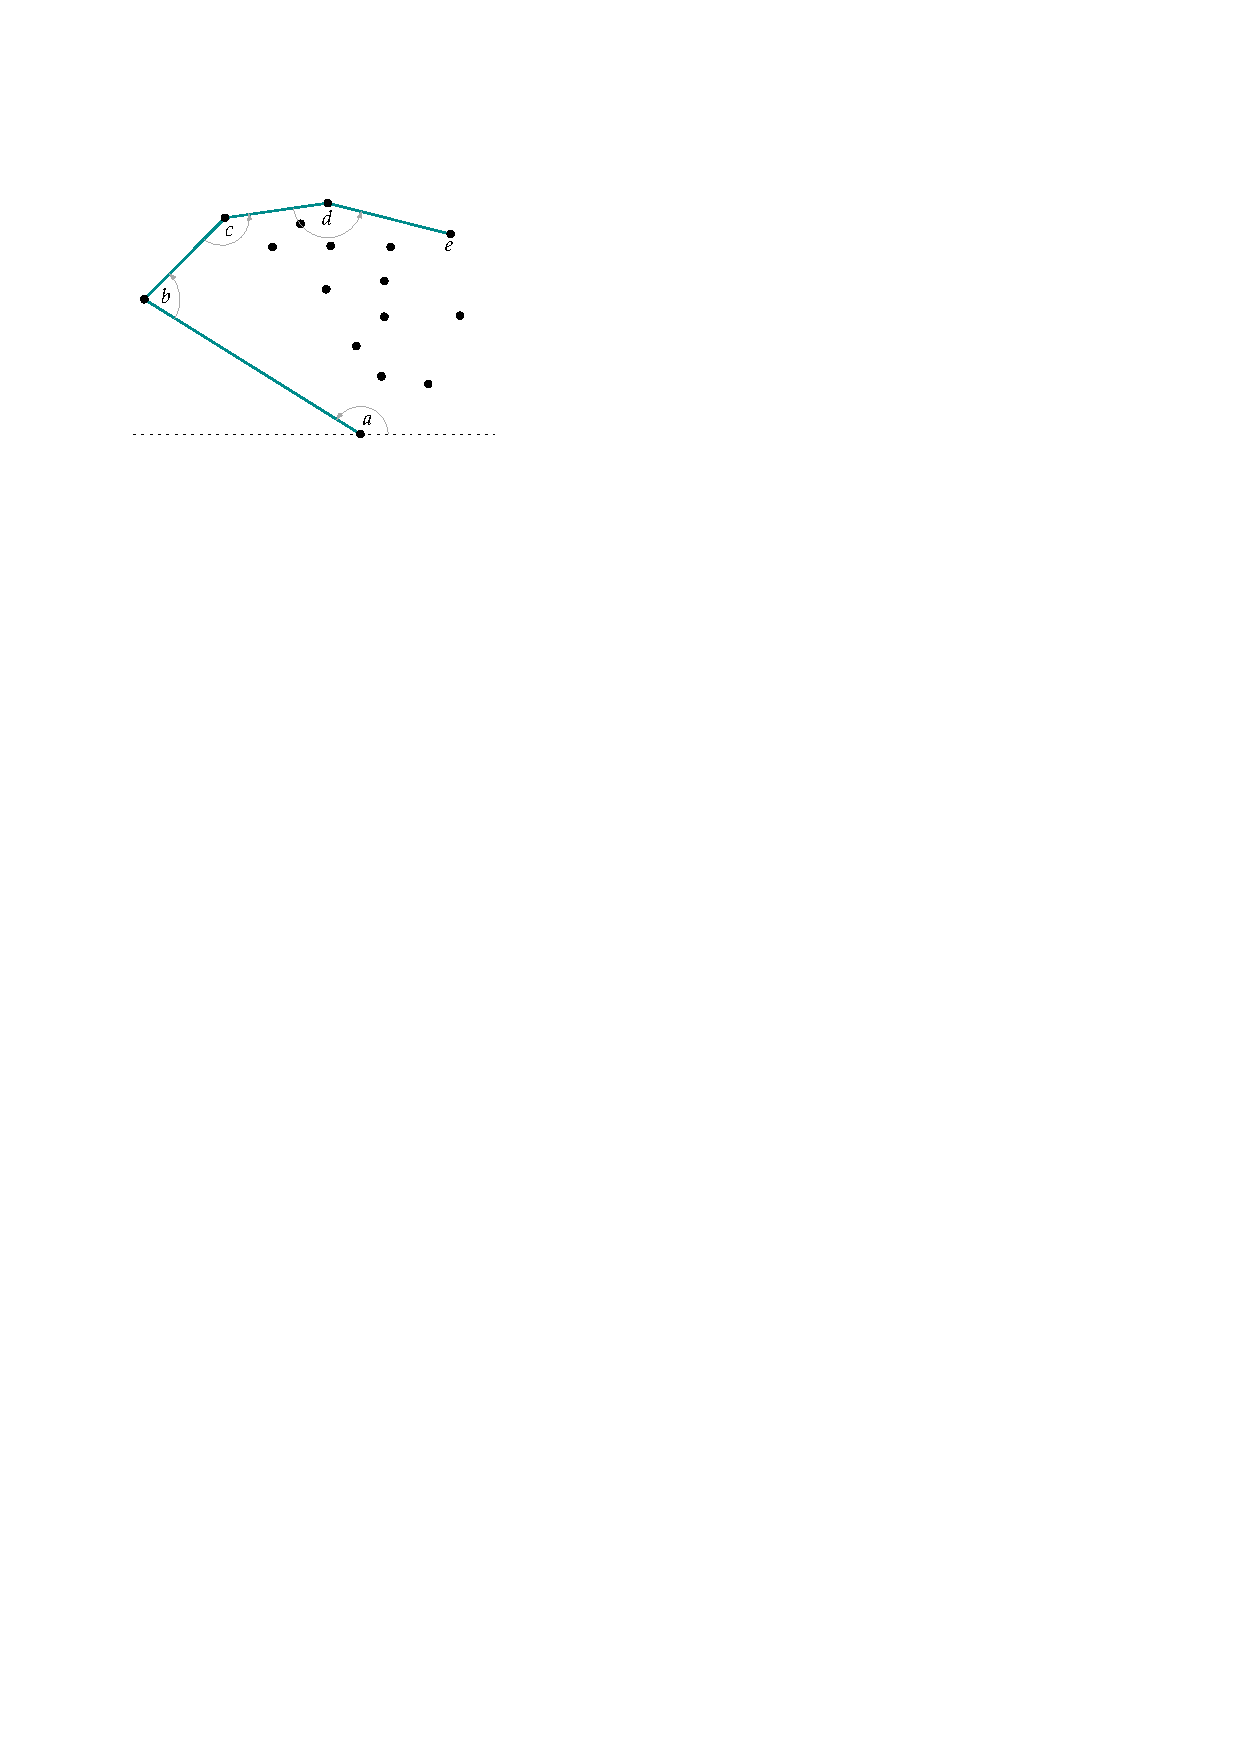
\includegraphics[page=1,width=\textwidth]{figs/giftwrapping.pdf}
    \caption{}
  \end{subfigure}%
  \qquad
  \begin{subfigure}[b]{0.3\linewidth}
    \centering
    \includegraphics[page=2,width=\textwidth]{figs/giftwrapping.pdf}
    \caption{}
  \end{subfigure}
  \caption{\textbf{(a)} First four steps of the gift wrapping algorithm to compute the convex hull. \textbf{(b)} The resulting convex hull.}
\label{fig:giftwrapping}
\end{figure}
It begins with a point that is guaranteed to be on conv($S$) (we can take an `extreme', such as $a$ in Figure~\ref{fig:giftwrapping} that is the point with the lowest $y$-coordinate), and then picks the point in $S$ (omitting the ones already on conv($S$)) for which the polar angle between the horizontal line and that point (at $a$) is the smallest ($b$ in this case), and adds it to conv($S$).
Then for $b$, the polar angle is calculated from the line $ab$; and the algorithm continues this way until $a$ is visited again.

%
Properties:
\\
\begin{tabular}{@{}ll@{}}
\toprule
P1. & The sole polygon is guaranteed to be regular (and convex).  \\  
% P2. & A subset of $S$, or all of them, forms the region. \\ 
P2. & All points are on or inside the region. \\ 
P3. & One component.  \\ 
P4. & No holes in the region.  \\  
\bottomrule
\end{tabular}



%%%%%%%%%%%%%%%%%%%%
%
\section{Moving arm}

\paragraph{Arm of length $l$.} 
The moving arm is a generalisation of the gift wrapping algorithm where the infinite line, used to calculate the polar angles, is replaced by a line segment of a given length $l$ (the ``moving arm'').
This means that, unlike the original gift wrapping algorithm, only a subset of the points in $S$ are considered at each step.
This also means that potentially the result is a polygon that is not convex.
Figure~\ref{fig:movingarm}a shows the first few steps for a given $l$, and it can be observed that 1 point is not part of the final region (.
Observe that if $l$ had been larger then the convex of $S$ could have been obtained.
\begin{figure}
  \centering
  \begin{subfigure}[b]{0.3\linewidth}
    \centering
    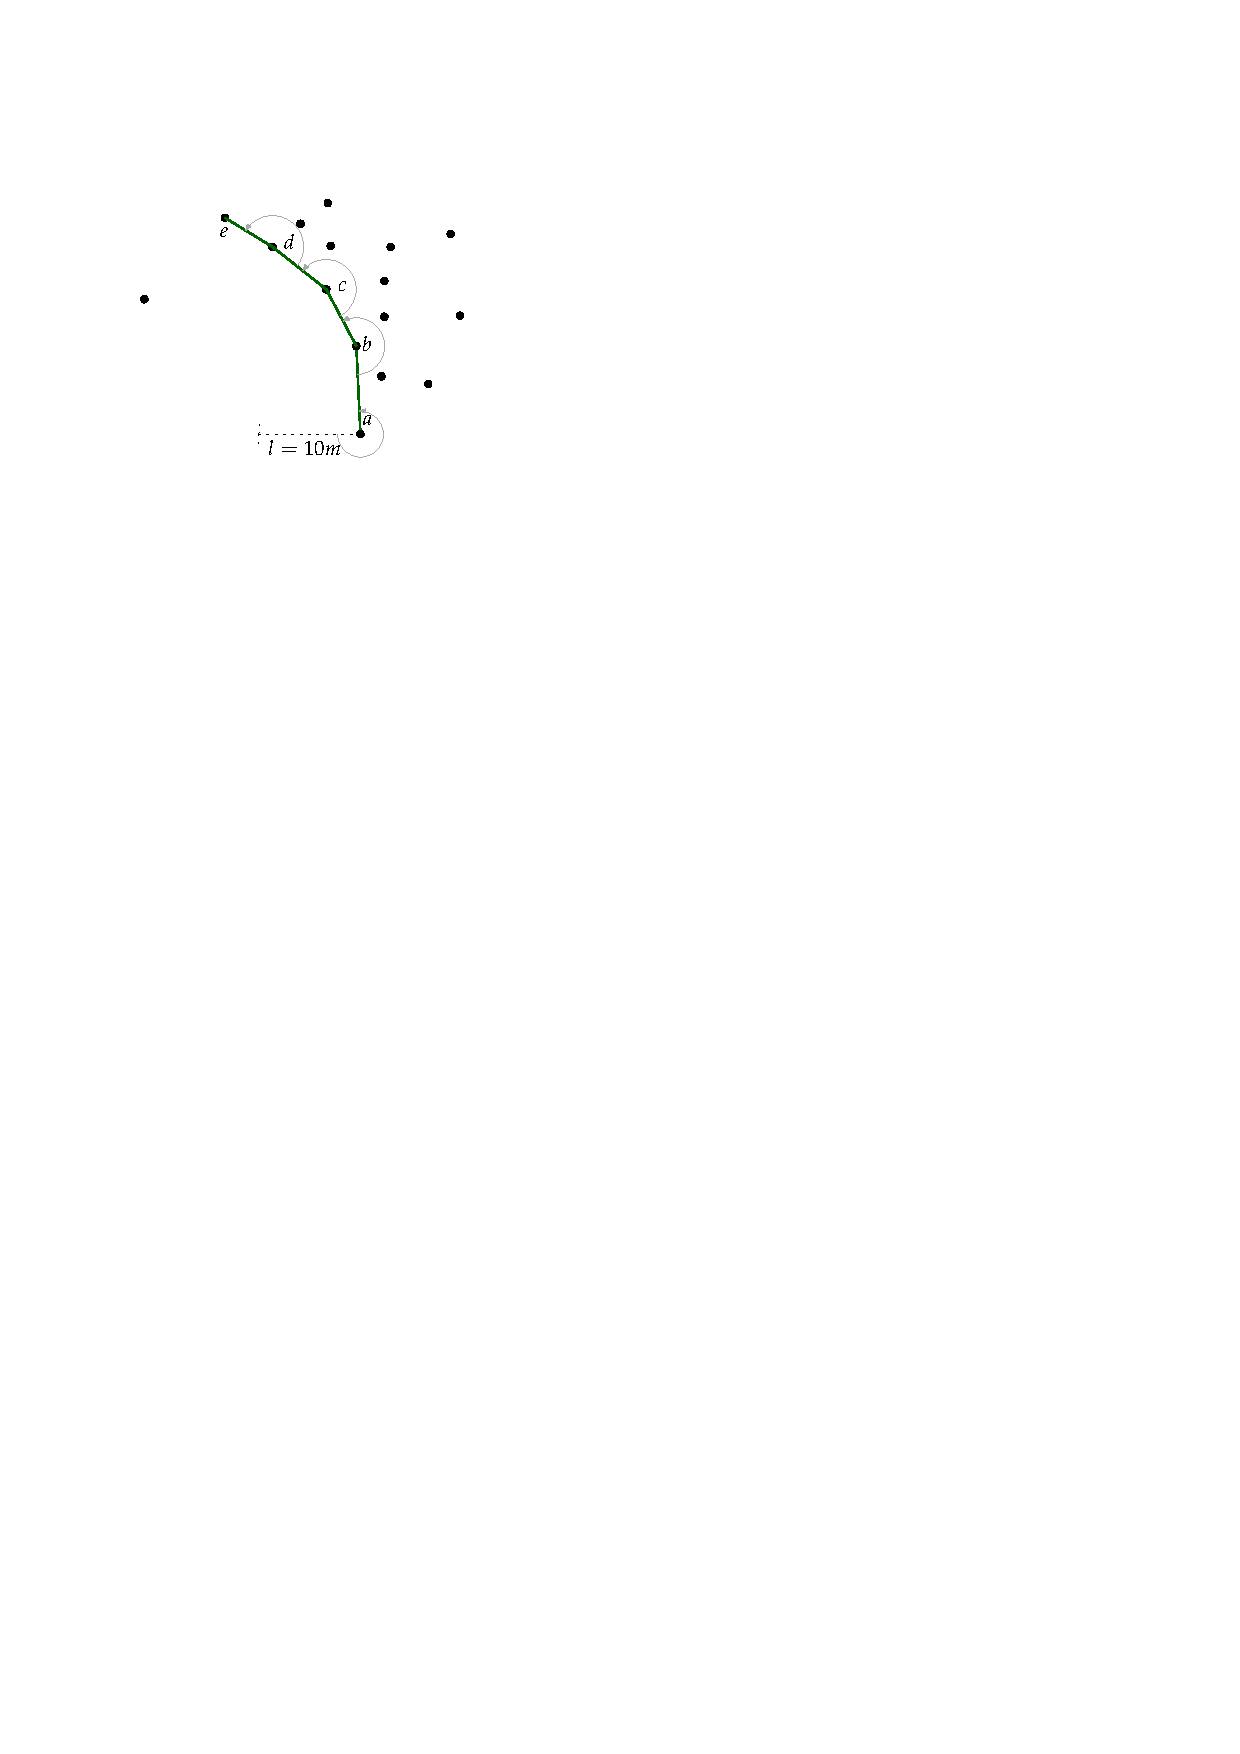
\includegraphics[page=1,width=\textwidth]{figs/movingarm.pdf}
    \caption{}
  \end{subfigure}%
  \qquad 
  \begin{subfigure}[b]{0.3\linewidth}
    \centering
    \includegraphics[page=2,width=\textwidth]{figs/movingarm.pdf}
    \caption{}
  \end{subfigure}
  \qquad 
  \begin{subfigure}[b]{0.3\linewidth}
    \centering
    \includegraphics[page=3,width=\textwidth]{figs/movingarm.pdf}
    \caption{}
  \end{subfigure}
  \caption{\textbf{(a)} First four steps of the \emph{moving arm algorithm} (with a lenght $l$) to compute the spatial extent. \textbf{(b)} First four steps of the \emph{moving arm algorithm} (with a \emph{knn} where $k=3$) to compute the spatial extent. \textbf{(c)} The resulting region is the same for both, and it is concave. Observe that 1 point from $S$ (highlighted in red) is not part of the concave region.}
\label{fig:movingarm}
\end{figure}

%

\paragraph{Adaptative arm with \emph{knn}} 
There exists a variation of this algorithm where the moving arm has an adaptative length at each step: the $k$ nearest neighbours (knn) of a given point $p$ are used instead.
As can be seen in Figure~\ref{fig:movingarm}b, the largest polar angle, as used for gift wrapping algorithm, is used to select the point at each step.

%

\paragraph{No guarantee to work.} 
Both versions of the algorithm will work in most cases, but there are no guarantee that they will for all input.
Figure~\ref{fig:movingarm_kdd} shows a concrete example.
\begin{figure}
  \centering
  \begin{subfigure}[b]{0.3\linewidth}
    \centering
    \includegraphics[page=4,width=\textwidth]{figs/movingarm.pdf}
    \caption{}
  \end{subfigure}
  \qquad
  \begin{subfigure}[b]{0.3\linewidth}
    \centering
    \includegraphics[page=5,width=\textwidth]{figs/movingarm.pdf}
    \caption{}
  \end{subfigure}
\caption{Moving arm with \emph{kdd} when $k=4$. \textbf{(a)} When the point $e$ is being processed, $f$ is the next one chosen. \textbf{(b)} From $f$, no other points can be chosen since the resulting region would be self-intersecting.}
\label{fig:movingarm_kdd}
\end{figure}
A solution to this problem would be in this case to either choose another $k$, or to rotate counter-clockwise instead of clockwise, which will in practice yield different results.


%
\paragraph{Different clusters?} 
One drawback of the moving arm method is that only one polygon is output.
While this can be useful to discrard unwanted outliers, if $S$ is distributed and forms different clusters (see for instance Figure~\ref{fig:clusters}a, then only the cluster that is the `lowest' (since the lowest point is picked as a starting point) will be output for the region.
\begin{figure}
  \centering
  \begin{subfigure}[b]{0.35\linewidth}
    \centering
    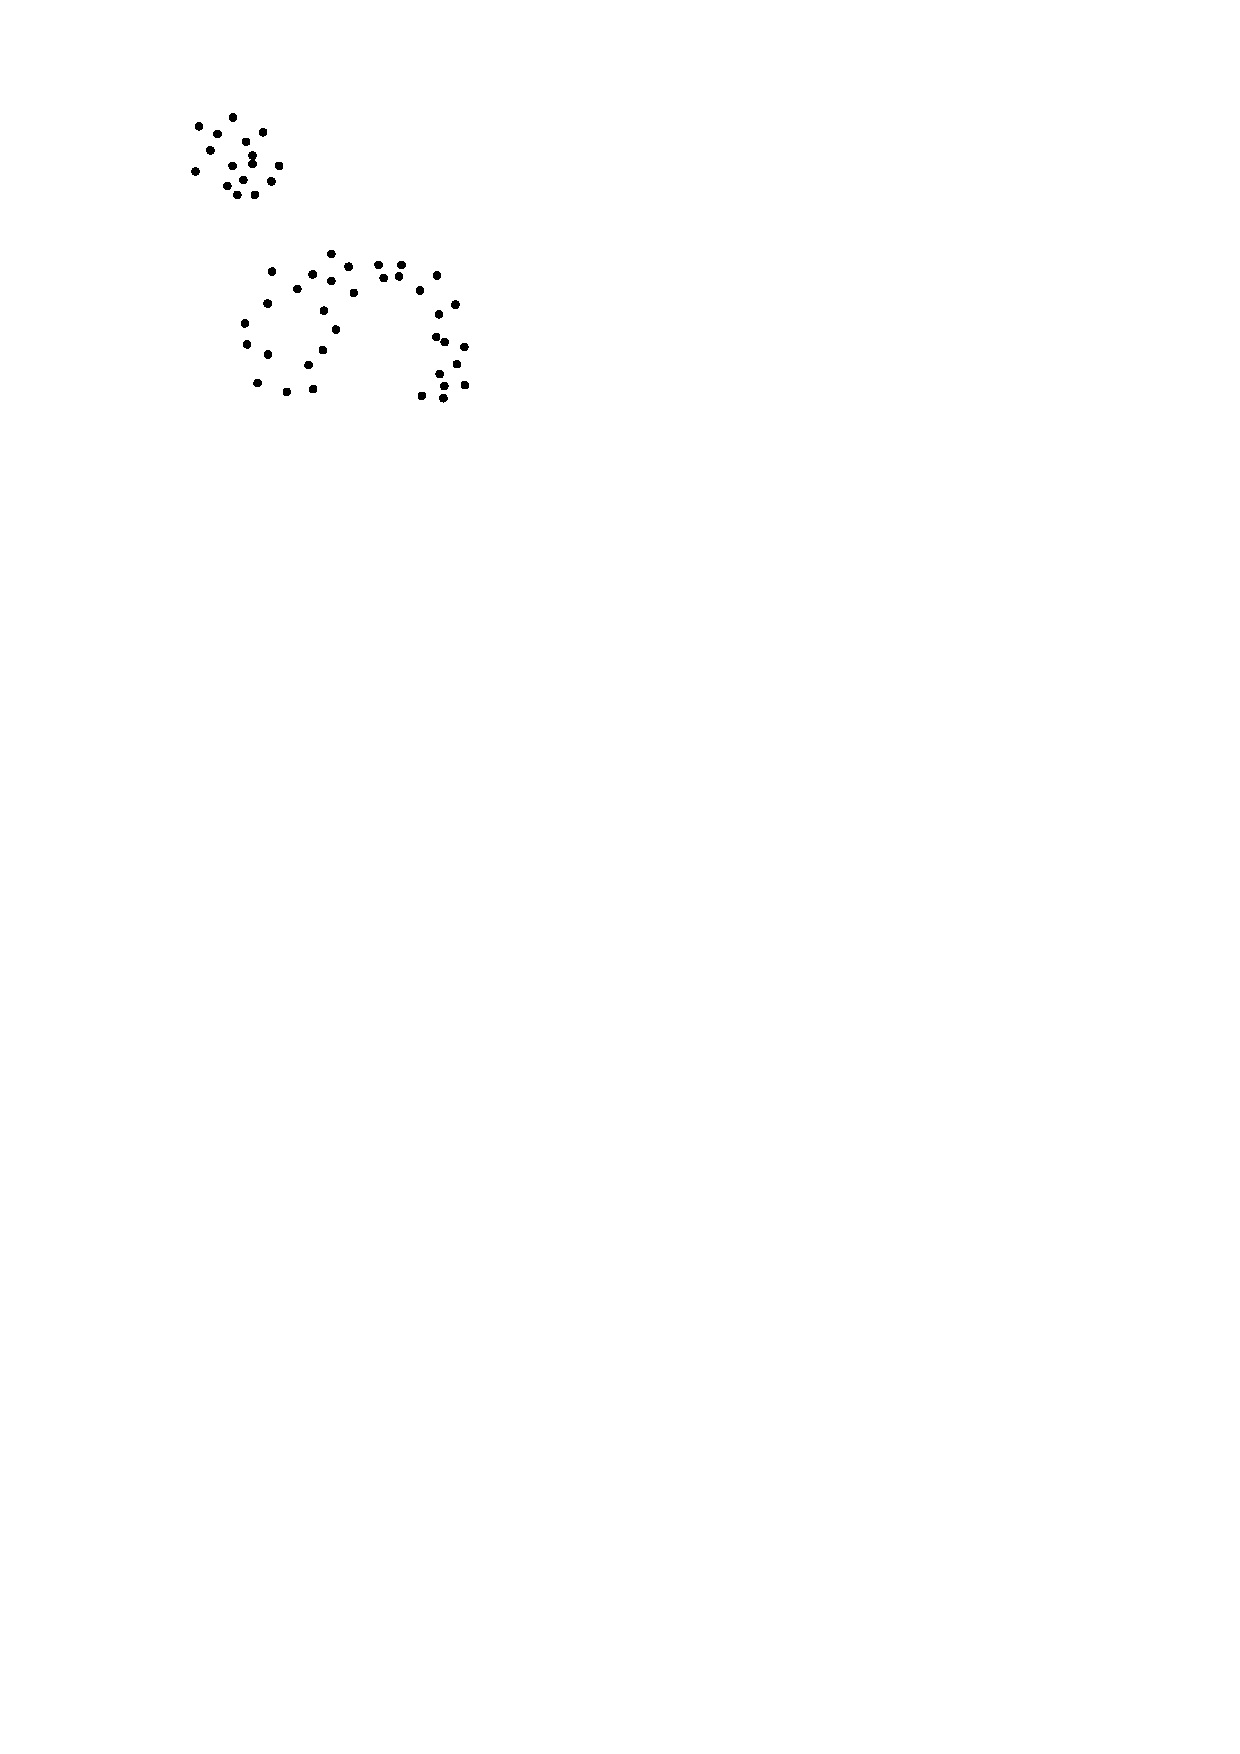
\includegraphics[page=1,width=\textwidth]{figs/clusters.pdf}
    \caption{}
  \end{subfigure}
  \qquad \qquad
  \begin{subfigure}[b]{0.35\linewidth}
    \centering
    \includegraphics[page=2,width=\textwidth]{figs/clusters.pdf}
    \caption{}
  \end{subfigure}
\caption{\textbf{(a)} $S$ has two distinct clusters. {(b)} Typical output if $S$ processed as a single cluster with a moving arm algorithm.}
\label{fig:clusters}
\end{figure}
In practice, when it is the case, the input points are sometimes first preprocessed with a clustering algorithm (in the case of Figure~\ref{fig:clusters}a two clusters should be detected) and then each cluster is processed independently.

%

Properties:
\\
\begin{tabular}{@{}ll@{}}
\toprule
P1. & The sole polygon could be degenerate (self-intersection).  \\  
% P2. & A subset of $S$, or all of them, forms the region. \\ 
P2. & Outliers can be discarded. \\ 
P3. & One component.  \\ 
P4. & No holes in the region.  \\  
\bottomrule
\end{tabular}



%%%%%%%%%%%%%%%%%%%%
%
\section{$\chi$-shape}

The $\chi$-shape is based on first constructing the Delaunay triangulation (DT) of $S$, and then removing iteratively the longest edge forming the envelop (at first this envelop is conv($S$)) until no edge is longer than a given threshold $l$.
The idea is to construct one polygon that is potentially non-convex, and that contains all the points in $S$.
Before removing an edge, we must verify that it will not introduce a topological issue in the envelop, that is that the envelop will not contain a self-intersection (see Figure~\ref{fig:chishape}c).
\begin{figure}
  \centering
  \begin{subfigure}[b]{0.25\linewidth}
    \centering
    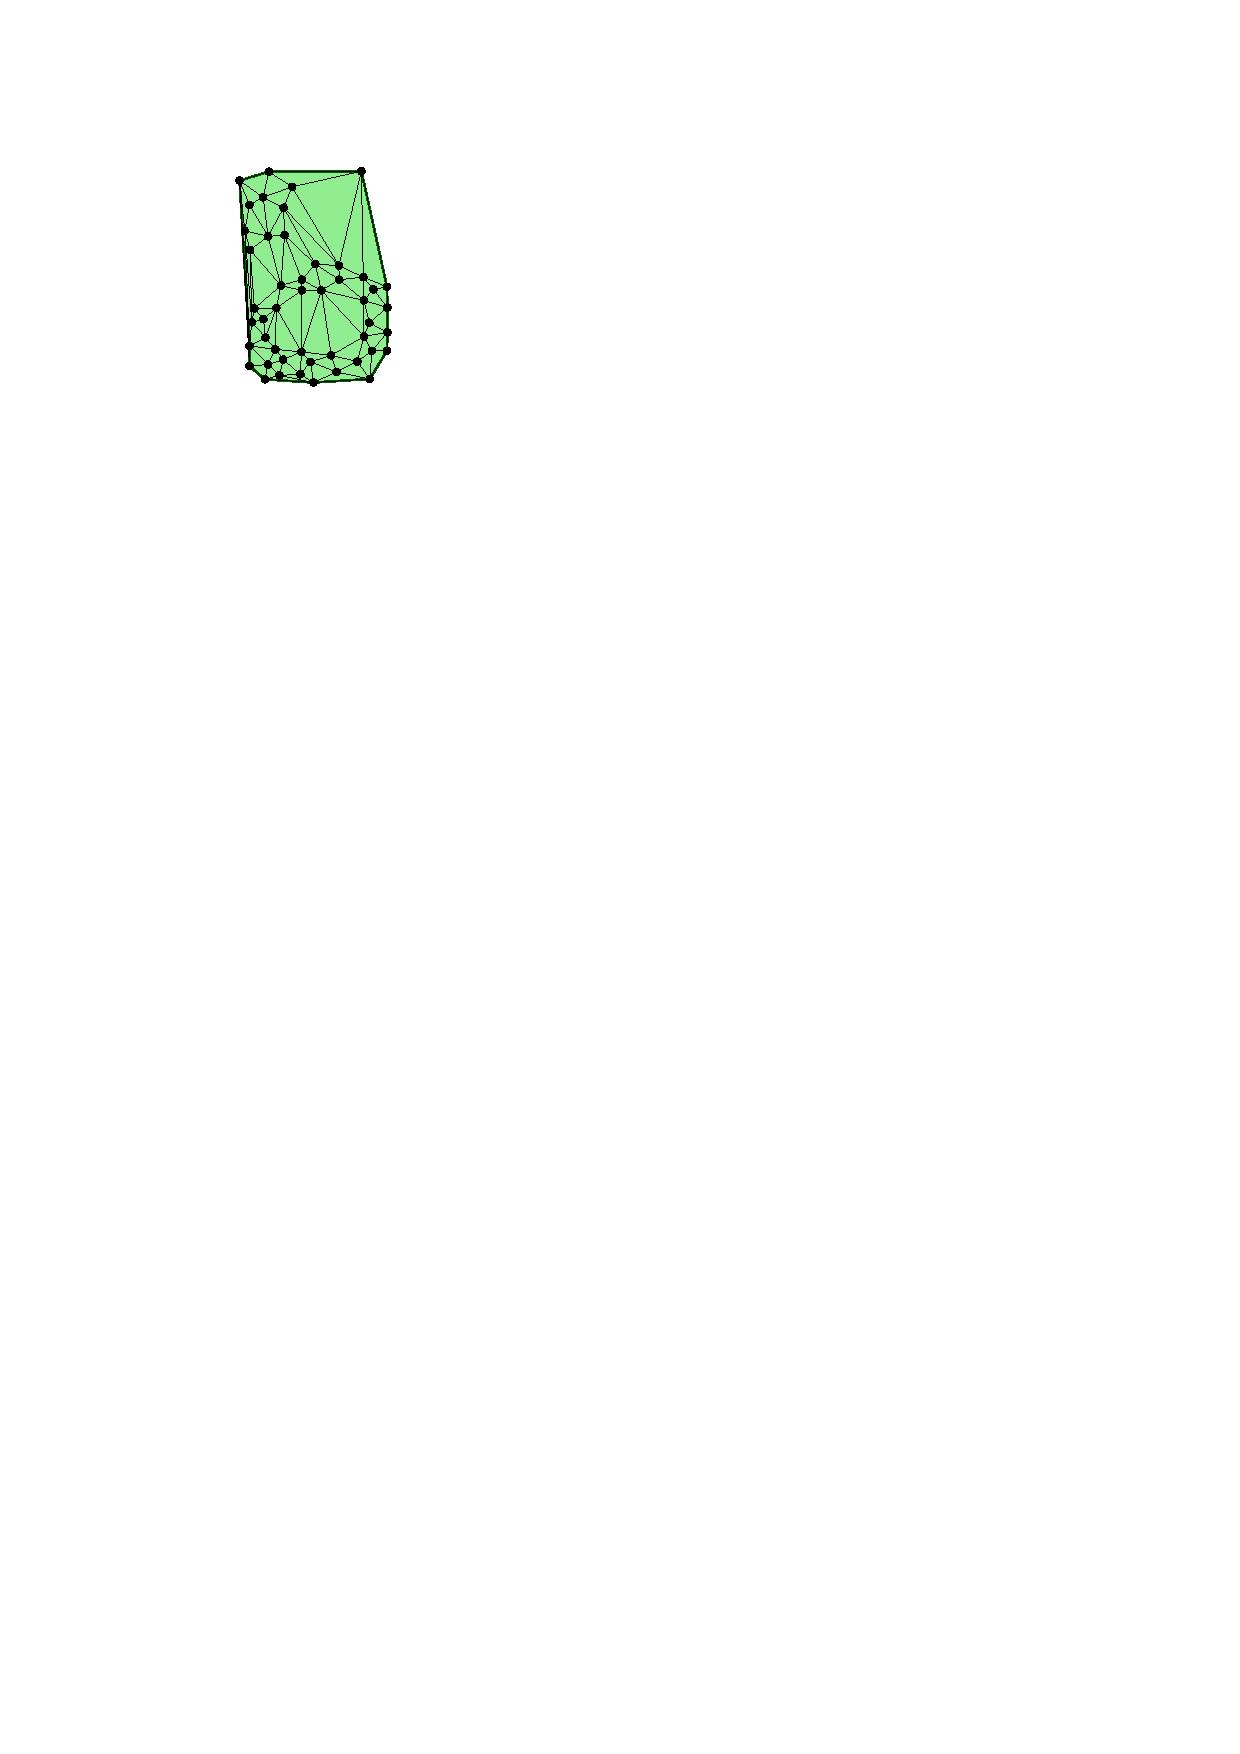
\includegraphics[page=1,width=\textwidth]{figs/chishape.pdf}
    \caption{}
  \end{subfigure}
  \qquad 
  \begin{subfigure}[b]{0.25\linewidth}
    \centering
    \includegraphics[page=2,width=\textwidth]{figs/chishape.pdf}
    \caption{}
  \end{subfigure}
  \qquad 
  \begin{subfigure}[b]{0.25\linewidth}
    \centering
    \includegraphics[page=3,width=\textwidth]{figs/chishape.pdf}
    \caption{}
  \end{subfigure}
\caption{$\chi$-shape examples. \textbf{(a)} $S$, its DT, and its envelope (cons($S$)). \textbf{(b)} After some edges have been removed. \textbf{(c)} The final result for a given threshold.}
\label{fig:chishape}
\end{figure}

%

Properties:
\\
\begin{tabular}{@{}ll@{}}
\toprule
P1. & The sole polygon is guaranteed to be regular.  \\  
% P2. & A subset of $S$, or all of them, forms the region. \\ 
P2. & All points are part of the region \\ 
P3. & One component.  \\ 
P4. & No holes in the region.  \\  
\bottomrule
\end{tabular}


%%%%%%%%%%%%%%%%%%%%
%
\section{$\alpha$-shape}

The $\alpha$-shape is conceptually a generalisation of the convex hull of a set $S$ of points.
% The $\alpha$-shape has stronger mathematical foundations then the alternatives mentioned above, and conceptually, it is a generalisation of the convex hull of a set $S$ of points.
% While the concepts are valid in any dimension, let us explain it here for the two-dimensional case.

%

It is best understood with the following analogy.
First imagine that $\mathbb{R}^2$ is filled with Styrofoam and that the points in $S$ are made of hard material.
Now imagine that you have a carving tool which is a circle of radius $\alpha$, and that this tool can be used anywhere from any direction (it is `omnipresent'), and that it is only stopped by the points.
The result after carving, called $\alpha$-hull, is one or more pieces of Styrofoam.
If we straighten the circular edges then we obtain the $\alpha$-shape.

%

Now let $\alpha$ be a real number with $0 \leq \alpha \leq \infty$.
If $\alpha = \infty$, then $\alpha$-shape is conv($S$); because you will not be able to carve inside conv($S$).
As $\alpha$ decreases, the $\alpha$-shape shrinks and cavities can appear, and different components can be created.
If $\alpha = 0$ then the $\alpha$-shape is $S$.

%

The $\alpha$-shape is not a polygon or a region, but a complex formed of $k$-simplices, where $0 \leq k \leq 2$.
Furthermore, it is a subcomplex of the Delaunay triangulation (DT) of $S$.
That is, the easiest method to construct an $\alpha$-shape is by constructing DT($S$), and then remove all edges that are shorter then $2\alpha$.

In practice, all the $\alpha$-shapes of $S$ (for different values of $\alpha$) can be calculated and discretised since we know that $\alpha$ will range from the shortest edge to the longest.
For each $k$-simplex, we can thus assign a range where it will be present.
% TODO : write this?
Implementations of the $\alpha$-shape will also offer to compute automatically an $\alpha$ such that the complex obtain is for instance connected and contains only one polygon.
\begin{figure}
  \centering
  \begin{subfigure}[b]{0.15\linewidth}
    \centering
    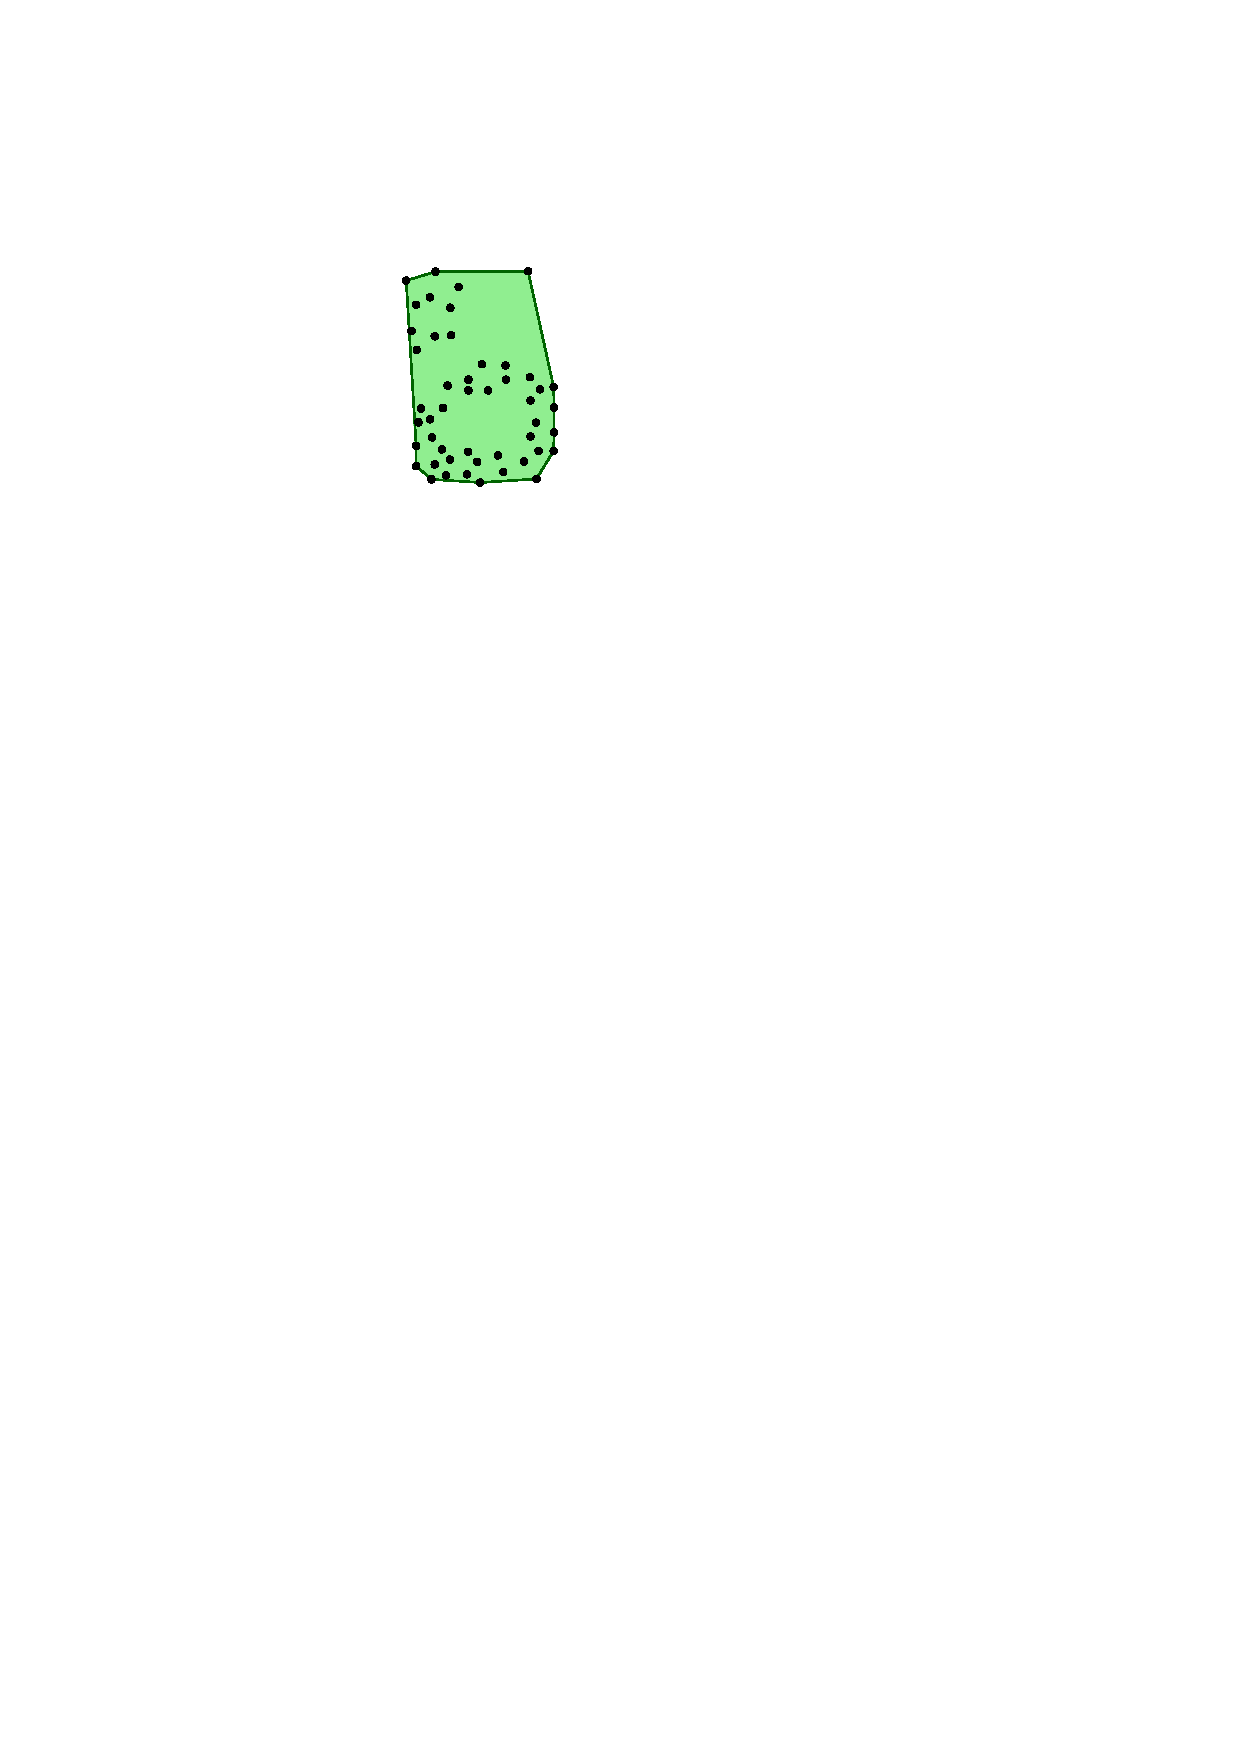
\includegraphics[page=1,width=\textwidth]{figs/alphashape.pdf}
    \caption{}
  \end{subfigure}
  \qquad 
  \begin{subfigure}[b]{0.15\linewidth}
    \centering
    \includegraphics[page=2,width=\textwidth]{figs/alphashape.pdf}
    \caption{}
  \end{subfigure}
  \qquad 
  \begin{subfigure}[b]{0.15\linewidth}
    \centering
    \includegraphics[page=3,width=\textwidth]{figs/alphashape.pdf}
    \caption{}
  \end{subfigure}
  \qquad 
  \begin{subfigure}[b]{0.15\linewidth}
    \centering
    \includegraphics[page=4,width=\textwidth]{figs/alphashape.pdf}
    \caption{}
  \end{subfigure}
  \qquad 
  \begin{subfigure}[b]{0.15\linewidth}
    \centering
    \includegraphics[page=5,width=\textwidth]{figs/alphashape.pdf}
    \caption{}
  \end{subfigure}
  \qquad 
\caption{$\alpha$-shape for different $\alpha$ decreasing values.}
\label{fig:alphashape}
\end{figure}

Properties:
\\
\begin{tabular}{@{}ll@{}}
\toprule
P1. & A complex of $k$-simplices.  \\  
% P2. & A subset of $S$, or all of them, are on the boundary of the region. \\ 
P2. & Some points can be omitted. \\ 
P3. & Several components possible.  \\ 
P4. & Regions can contain holes.  \\  
\bottomrule
\end{tabular}



%%%%%%%%%%%%%%%%%%%%
%
\section{Notes \& comments}

The properties listed in Section~\ref{sec:properties} are taken, and slightly adapted, from \citet{Galton06}. 

The gift wrapping algorithm to compute the convex hull of a set of points in $\mathbb{R}^2$ is from \citet{Jarvis73}.

The moving arm with a lenght is described in \citet{Galton06}, and the adaptative one in \citet{Moreira07}.
The authors describe different strategy to avoid make the algorithm works for all input, but these do not have any warranty to output a simple polygon.

The $\chi$-shape is from \citet{Duckham08}.

The explanation of the $\alpha$-shape is taken from \citet{Edelsbrunner94} and from CGAL documentation\footnote{\url{https://doc.cgal.org/latest/Alpha_shapes_2/index.html}}.

% TODO 
% https://en.wikipedia.org/wiki/DBSCAN
% https://en.wikipedia.org/wiki/Gift_wrapping_algorithm#/media/File:Animation_depicting_the_gift_wrapping_algorithm.gif

%%%%%%%%%%%%%%%%%%%%
%
\section{Exercises}

\begin{enumerate}
  \item What are the disadvantages of the $\chi$-shape compared with the $\alpha$-shape?
  \item If the parameter $l$ for the $\chi$-shape is equal to the $\alpha$ parameter, will the resulting shape be the same? compared with the $\alpha$-shape?
  \item Given an $\alpha$-shape of $S$, how to calculate how many components are part of it? 
  \item Given a DT($S$), how to extract conv($S$)?
  \item Draw what would happen if one of the 2 edges was removed in Figure~\ref{fig:chishape}c.
  \item What is the influence of $k$ for the moving arm algorithm (with a \emph{kdd})? Will a higher $k$ create a larger or smaller region in general?
\end{enumerate}


